\documentclass[11pt,a4paper]{article}
\usepackage[margin=21mm]{geometry}
\usepackage[T1]{fontenc}
\usepackage[utf8]{inputenc}
\usepackage{lmodern}
\usepackage{microtype}
\usepackage{booktabs,tabularx,array,multirow,makecell}
\usepackage{graphicx}
\usepackage{float}
\usepackage{subcaption}
\usepackage{amsmath,amssymb}
\usepackage{xcolor}
\usepackage{enumitem}
\usepackage{seqsplit}
\usepackage{xurl}
\usepackage{tikz}
\usetikzlibrary{arrows.meta,positioning}
\usepackage{listings}
\usepackage[hidelinks]{hyperref}
\usepackage{fancyhdr}
\usepackage{placeins}

\graphicspath{{../figures/}}

\definecolor{navy}{HTML}{16324F}
\definecolor{teal}{HTML}{007F82}
\definecolor{pale}{HTML}{F0F5F8}
\definecolor{amber}{HTML}{D97706}
\definecolor{coral}{HTML}{DC2626}
\definecolor{mint}{HTML}{059669}
\definecolor{slate}{HTML}{64748B}

\lstdefinelanguage{iecst}{
  morekeywords={FUNCTION_BLOCK,END_FUNCTION_BLOCK,VAR_INPUT,VAR_OUTPUT,VAR_IN_OUT,VAR,END_VAR,
    TYPE,STRUCT,END_STRUCT,END_TYPE,IF,THEN,ELSIF,ELSE,END_IF,CASE,OF,END_CASE,FOR,TO,DO,END_FOR,
    WHILE,END_WHILE,EXIT,RETURN,TRUE,FALSE,AND,OR,NOT,XOR,MOD,BOOL,INT,DINT,UDINT,UINT,USINT,
    REAL,LREAL,WORD,DWORD,TIME,LTIME,STRING,ARRAY,VARIANT},
  sensitive=false,
  morecomment=[s]{(*}{*)},
  morecomment=[l]{//},
  morestring=[b]'
}

\lstset{
  language=iecst,
  basicstyle=\ttfamily\small,
  keywordstyle=\bfseries\color{navy},
  commentstyle=\itshape\color{slate},
  stringstyle=\color{teal},
  breaklines=true,
  backgroundcolor=\color{pale},
  frame=single,
  rulecolor=\color{teal},
  columns=fullflexible,
  keepspaces=true,
  xleftmargin=2mm,
  xrightmargin=2mm
}

\setlist[itemize]{nosep,leftmargin=1.4em,itemsep=2pt}
\setlist[enumerate]{nosep,leftmargin=1.4em,itemsep=2pt}
\setlength{\parindent}{0pt}
\setlength{\parskip}{4.5pt}
\setlength{\headheight}{14pt}

\pagestyle{fancy}
\fancyhf{}
\fancyhead[L]{\small\color{slate} STAR: Industrial PLC Structured Text Agent}
\fancyhead[R]{\small\color{slate} Course Final Project Report}
\fancyfoot[C]{\small\thepage}

\newcommand{\pathcode}[1]{\nolinkurl{#1}}
\DeclareRobustCommand{\code}[1]{\texttt{\small\detokenize{#1}}}
\pdfstringdefDisableCommands{\def\code#1{\detokenize{#1}}\def\pathcode#1{\detokenize{#1}}}
\newcommand{\tbd}{\textcolor{amber}{\textbf{[TBD]}}}
\newcolumntype{L}[1]{>{\raggedright\arraybackslash}p{#1}}
\newcolumntype{Y}{>{\raggedright\arraybackslash}X}

\title{%
  {\color{navy}\Large\bfseries STAR: A Decoupled Agent Framework for Industrial IEC~61131-3 Structured Text Synthesis}\\[6pt]
  {\large\color{teal} Benchmark Construction, Scan-Aligned Formal Verification, and Controlled CODESYS~V3.5 Evaluation}
}
\author{Generative AI Course Final Project}
\date{14 November 2026}

\begin{document}
\maketitle

\begin{abstract}
Automatic synthesis of IEC~61131-3 Structured Text (ST) for industrial programmable logic controllers (PLCs) differs sharply from general-purpose software generation: candidate programs must conform to deterministic scan-cycle execution, retain internal edge and timer state across cycles, enforce same-scan safety preemption, and satisfy platform-specific CODESYS~V3.5 compiler and static-analysis contracts. Moreover, code that compiles and passes finite test suites can still conceal single-scan mode-transition delays or priority regressions. This work presents an end-to-end engineering methodology and full 128-run empirical evaluation spanning three pillars: (1) a frozen 32-task benchmark (\code{normalized-20261114}, \code{dataset_sha256: d305f96c...}) combining 20 verbatim public tasks (\code{PUB001}--\code{PUB020}) and 12 AI-assisted, human-reviewed independent synthesis tasks (\code{SELF001}--\code{SELF012}), paired with 276 held-out fixed test cases (2,994 scan steps), 294 end-of-scan-aligned LTL specifications, and positive/negative dual-control \code{.smv} verification (32/32 reference models proven true; 32/32 mutant controls refuted); (2) \textbf{STAR}, a decoupled, leak-free agent harness combining a four-stage scan contract planner, relevance-ranked dialect cards, hash-guarded compiler repair, assertion-isolated in-loop symbolic verification (\code{Scheme A}, \code{ST->SMV} over \code{NuSMV} BDD and \code{nuXmv} SMT), and anti-lazy lexicographic ratchet simulation repair; and (3) a symmetric $2 \times 2$ benchmark comparing unmodified \code{Codex CLI v0.142.5} (\textbf{E1}, \textbf{E2}) against \textbf{STAR} (\textbf{E3}, \textbf{E4}) across \code{deepseek-v4.1-flash-1017} and \code{gpt-6.1-terra} under uniform maximum reasoning effort (\code{reasoning.effort = "high"}) and shared quotas. On \code{deepseek-v4.1-flash-1017}, \textbf{STAR} (\textbf{E3}) eliminates dialect collisions, elevating final compilation from \textbf{E1}'s 28/32 (87.5\%) to \textbf{32/32 (100\%)}, increasing evaluated fixed-case passes from 196/208 (94.2\%) to \textbf{226/238 (95.0\%, 81.9\% of all 276 planned cases)} and task-level passes from 23/32 to \textbf{27/32}, while compressing cumulative context input nearly 11-fold (4.74M down to 433k tokens). On \code{gpt-6.1-terra}, unmodified \code{Codex CLI} (\textbf{E2}) achieves 29/32 (90.6\%) compilation, the highest evaluated case pass rate (\textbf{220/222 = 99.1\%}), 27/32 task pass, and 18 Stage~3 formal \code{PASS} verdicts with compact outputs (72.8k tokens, \textyen 5.21), whereas \textbf{STAR} (\textbf{E4}) matches \textbf{18} formal passes and 98.2\% (217/221) evaluated cases using fewer inputs (366k tokens) but higher structured output cost (\textyen 7.38) alongside three pre-patch compiler-lock timeouts. Finally, symbolic checking uncovers single-scan transition and exclusion defects in both \textbf{E3} (\code{PUB011}, passing 8/8 fixed tests) and \textbf{E1} (\code{PUB020}, passing 11/11 fixed tests), empirically validating dual runtime and formal verification.
\end{abstract}

\section{Introduction and Problem Statement}

\subsection{Industrial Control Background and Core Challenges}
Programmable logic controllers (PLCs) execute sequential interlocks, mode arbitration, timing supervision, and continuous regulation across manufacturing lines using IEC~61131-3 languages, with Structured Text (ST) serving as the primary high-level textual notation. Unlike stateless function evaluation in general software engineering, controller correctness depends on cyclic scan-cycle semantics and strict safety guarantees:
\begin{enumerate}
  \item \textbf{Single-Scan Sampling and Persistent State}: Each \code{FUNCTION_BLOCK} invocation samples external inputs once per cycle, reconciles them against retained pre-scan internal state (edge memories, latches, timers), and updates outputs deterministically. Built-in stateful blocks such as \code{TON}, \code{TOF}, \code{TP}, \code{R_TRIG}, and \code{F_TRIG} must execute unconditionally on the top-level scan path rather than inside conditional branches where skipped calls freeze internal elapsed timers or edge histories.
  \item \textbf{Same-Scan Safety Preemption and Dialect Contracts}: Emergency stops and protection interlocks must override motor or actuator commands within the exact scan cycle they assert. In addition, industrial deployment requires satisfying target compiler rules and static-analysis checks (\code{CODESYS V3.5 SP22 Patch 4}), including caller-owned \code{VAR_IN_OUT} composite storage, \code{ARRAY[*]} variable-length bounds, 0-based \code{STRING} element indexing, nanosecond \code{LTIME} literals, and \code{VARIANT} reflection.
  \item \textbf{Insufficiency of Compilation and Finite Testing}: Large language models frequently emit syntactically valid ST code that compiles cleanly and passes representative test cases, yet fails on unobserved edge combinations---such as asserting a manual start signal on the exact rising scan where operating mode switches from manual to automatic.
\end{enumerate}

\subsection{Research Objectives and Scope Alignment}
Table~\ref{tab:objectives} maps the core engineering objectives and deliverables of this project to their implemented artifacts and current evaluation status.

\begin{table}[htbp]
\centering
\caption{Alignment of core project objectives, artifacts, and verification status as of 14 November 2026.}
\label{tab:objectives}
\footnotesize
\begin{tabularx}{\textwidth}{@{}L{0.23\textwidth}L{0.34\textwidth}Y@{}}
\toprule
\textbf{Project Dimension} & \textbf{Core Technical Requirement} & \textbf{Implemented Artifacts \& Current Status} \\
\midrule
\textbf{Benchmark \& LTL Specifications} & Curate official + independent tasks ($\ge 10$), preserve provenance, verify scan semantics & \textbf{Completed}: 32 tasks (20 verbatim public + 12 AI-generated, human-reviewed self-built); 276 cases, 2,994 scans, 294 LTLs; 32/32 reference and 32/32 mutant SMVs verified. \\
\textbf{STAR vs.\ Baseline Frameworks} & Compare self-designed harness against established tool-using baseline across $\ge 2$ models & \textbf{Completed}: Decoupled \textbf{STAR} harness vs.\ unmodified \code{Codex CLI v0.142.5} evaluated on \code{deepseek-v4.1-flash-1017} and \code{gpt-6.1-terra} at max reasoning. \\
\textbf{Simulation \& Formal Tooling} & Integrate real PLC compilation/simulation and symbolic model checking & \textbf{Completed}: Real CODESYS~SP22 compilation + 1\,ms cyclic simulation, 5-stage \code{ST->SMV} compiler (\code{NuSMV} BDD / \code{nuXmv} SMT), \code{ScanContract}, and WebUI. \\
\textbf{Controlled Empirical Evaluation} & Execute $2\times 2$ crossed matrix (128 runs), stratified analysis, deep-dive case studies & \textbf{Completed (128/128 Runs)}: All four groups (\textbf{E1}--\textbf{E4}, 32 tasks each) archived under unified \pathcode{batch.py} adjudication with cross-condition quantitative and case analysis. \\
\textbf{Cross-Platform Boundary} & Optional extension toward Siemens TIA Portal or secondary targets & \textbf{Scoped Boundary}: Deep validation focused on \code{CODESYS V3.5 SP22 Patch 4}, with decoupled backend interfaces reserved for future targets. \\
\bottomrule
\end{tabularx}
\end{table}

% Sections 2, 3, and 4: Toolchain, Dataset & LTL Alignment, STAR Framework, and WebUI/SMV Infrastructure

\section{Execution Environment, Toolchain, and Controlled Setup}

\subsection{Software Toolchain and Runtime Isolation}
All compilation and functional test runs execute against a real Windows installation of \code{CODESYS Development System 3.5.22.40} (\code{CODESYS V3.5 SP22 Patch 4}) driven via its embedded IronPython~2.7 Scripting Engine, with \code{CODESYS Static Analysis Light} active. Candidate function blocks are built inside copies of a hash-frozen template project (\pathcode{codesys/templates/benchmark.project}, device target \code{Control Win V3 x64}, \code{template_sha256}: \texttt{\small\seqsplit{70d40be7b4b9bdf4a22619a7ba47156422cf6beaec692480f0e5ee2acbda8909}}). Runtime functional evaluation drives the compiled \code{FB_Task} under a \code{1ms} cyclic \code{ScriptTaskObject} running a generated \code{PLC_PRG} harness over the local simulation target; no external physical PLC hardware is connected.

Formal verification is dispatched dynamically across two symbolic model checkers: \textbf{NuSMV~2.7.1} (BDD engine) for pure Boolean and bounded integer controllers, and \textbf{nuXmv} (with the \code{MathSAT} SMT backend, default BMC depth 25) for designs containing IEEE-754 floating-point ports (\code{REAL}/\code{LREAL}) or unbounded arithmetic. Software orchestration and offline regression suites run on Python~3.12+ inside a standard environment, while real CODESYS compilation and gateway-connected simulation run inside normal un-sandboxed Windows processes because restricted sandboxes block APInstaller event-log writes and gateway communication.

\subsection{Experimental Matrix and Reasoning Configuration}
Following \pathcode{configs/fullflow_matrix.json}, evaluation uses a crossed $2 \times 2$ design across two frameworks---the self-developed \textbf{STAR} harness (\pathcode{self_harness}) and unmodified official \textbf{Codex CLI~v0.142.5}---and two foundation models accessible through the project relay (\pathcode{deepseek-v4.1-flash-1017} and \pathcode{gpt-6.1-terra}), totaling 128 planned task runs across 32 benchmark tasks (Table~\ref{tab:matrix}). Crucially, \textbf{all four conditions uniformly enforce maximum reasoning strength} (\code{reasoning.effort = "high"} in every API payload), isolating architectural and model differences without varying inference effort. Pre-configured ablation modes (\code{no_planner}, \code{no_dialect}, \code{no_selftest}) are additionally preserved in \pathcode{configs/experiments.json} for follow-up attribution studies.

\begin{table}[htbp]
\centering
\caption{Controlled $2 \times 2$ benchmark matrix spanning agent frameworks and foundation models.}
\label{tab:matrix}
\footnotesize
\begin{tabularx}{\textwidth}{@{}llL{0.28\textwidth}Y@{}}
\toprule
\textbf{ID} & \textbf{Agent Framework} & \textbf{Model Route} & \textbf{Reasoning Effort \& Runtime Transport} \\
\midrule
\textbf{E1} & \textbf{Codex CLI (\code{v0.142.5})} & \pathcode{deepseek-v4.1-flash-1017} & Max (\code{reasoning.effort = "high"}), local \code{CodexTransport} HTTP relay + MCP server \\
\textbf{E2} & \textbf{Codex CLI (\code{v0.142.5})} & \pathcode{gpt-6.1-terra} & Max (\code{reasoning.effort = "high"}), local \code{CodexTransport} HTTP relay + MCP server \\
\textbf{E3} & \textbf{STAR (\code{self_harness})} & \pathcode{deepseek-v4.1-flash-1017} & Max (\code{reasoning.effort = "high"}), native multi-stage \code{ResponsesClient} \\
\textbf{E4} & \textbf{STAR (\code{self_harness})} & \pathcode{gpt-6.1-terra} & Max (\code{reasoning.effort = "high"}), native multi-stage \code{ResponsesClient} \\
\bottomrule
\end{tabularx}
\end{table}

\subsection{Shared Budgets, Quotas, and Engineering Guardrails}
Rather than treating operational limits as optimal universal constants, runtime quotas act as symmetric guardrails for fairness and cost containment across agents. As logged in each 14~November~2026 run's \pathcode{generation/runtime_config.json}:
\begin{itemize}
  \item \textbf{Symmetric Tool and Call Quotas}: Each task allows at most \code{max_repairs = 2} compile-repair iterations (initial draft plus up to 2 repairs, i.e., $\le 3$ builds), \code{max_verifications = 3} formal checks (capped at \code{60s} each), \code{max_simulations = 3} internal self-test simulation rounds, at most \code{9} LLM requests, and a cumulative \code{300,000}-token cap. For Codex CLI, standalone \pathcode{mcp_server.py} enforces identical tool counters and rejects excess calls with \code{isError: true}.
  \item \textbf{Timeouts, Output Caps, and Lock Budget Decoupling}: Per-task wall time was bounded at \code{task_timeout = 1800s} during the main campaign (raised to \code{2400s} by default in the latest codebase revision), with \code{compiler_timeout = 180s}, \code{llm_timeout = 420s}, single-turn output caps of \code{24,576} (Coder/Tester) and \code{32,768} (Planner/Repair) tokens, and a cumulative fee fuse of \code{reported_cost_stop_cny = 75}. Recent hardening further decoupled the shared CODESYS mutex wait budget (\code{compiler_lock_timeout = 960s}, dynamically extended for long-duration timed simulations) from the compiler execution timeout so concurrent workers waiting on the single-instance IDE do not trigger premature lock timeouts.
  \item \textbf{Baseline Context Adaptation (\code{codex_transport.py})}: Because Codex CLI injects its own system prompt and tool schemas, applying STAR's tighter input context cap causes immediate prompt truncation; the relay layer relaxes total input context clipping for Codex CLI while preserving identical output token limits, reasoning effort, tool quotas, and stop rules.
\end{itemize}

\section{Benchmark Dataset and Formal Specification Design}

\subsection{Provenance, Normalization, and Independent Review}
The frozen dataset release \code{normalized-20261114} (SHA-256: \texttt{\small\seqsplit{d305f96c2faaa87f60a24be90c00ad0b32153492e741b87547d132c591e0e9ee}}) contains \textbf{32 control tasks}:
\begin{enumerate}
  \item \textbf{20 Public Tasks (\code{PUB001}--\code{PUB020})}: Ten problems derive from the public course task pool (\code{PUB001}--\code{PUB010}) and ten from instructor supplementary tasks (\code{PUB011}--\code{PUB020}). Automated alignment (\pathcode{requirements/source_alignment.json}) against the original 25-page question bank (fingerprint \code{4ce56562...}) confirms a text sequence similarity of \code{1.0} and complete interface matching across all 20/20 problems. Ambiguities common in natural-language prompts (concurrent priority order, invalid input sanitization, out-of-bounds clamping, initial output defaults) are clarified additively via \code{scan_semantics}, \code{safety_priority}, \code{assumptions}, and \code{specification_contract} without modifying the verbatim English statements. All 32 tasks underwent bilingual human verification.
  \item \textbf{12 Self-Built Tasks (\code{SELF001}--\code{SELF012}, AI-Generated + Human Reviewed)}: Marked explicitly with provenance \code{independent_synthesis}, these tasks were authored through \textbf{AI-assisted generation followed by human review}. An AI assistant initially synthesized problem specs, boundary conditions, engineering \code{rationale}, and 7--12 fixed scan sequences covering multi-actuator interlocks, hysteresis tank control, alternating pump rotation, consecutive-scan qualification, bit-parity checks, and bounded fault retries while avoiding structural duplication of public tasks. Each candidate spec was exercised in Python against an independent reference transition model and then manually audited via a bilingual review view for disambiguation, initialization, priority resolution, recovery edges, and LTL alignment. This review establishes internal benchmark consistency and does not constitute formal IEC~61508 safety certification.
\end{enumerate}

\subsection{Industrial Control Semantics and Diversity Metrics}
The corpus enforces strict \code{FUNCTION_BLOCK FB_Task} ownership conventions separating read-only \code{VAR_INPUT}, \code{VAR_OUTPUT}, and caller-owned persistent \code{VAR_IN_OUT} references (e.g., multi-pump banks in \code{PUB007}, analog channels in \code{PUB008}, recipe structs in \code{PUB017}, generic FIFOs in \code{PUB018}). Timing coverage deliberately combines pure scan-counted discrete state machines across \code{SELF001}--\code{SELF012} (immune to host scheduling jitter) with 6 real-timer public problems (\code{PUB004}, \code{PUB005}, \code{PUB006}, \code{PUB010}, \code{PUB012}, \code{PUB013}) totaling 315 non-zero \code{dt_ms} scan intervals. Table~\ref{tab:dataset} and Figure~\ref{fig:dataset} summarize benchmark breadth across difficulty tiers, control patterns, IEC~61131-3 types, and test-trace scale.

\begin{table}[htbp]
\centering
\caption{Diversity profile of the normalized 32-task IEC~61131-3 benchmark (\code{normalized-20261114}).}
\label{tab:dataset}
\footnotesize
\begin{tabularx}{\textwidth}{@{}L{0.21\textwidth}L{0.48\textwidth}Y@{}}
\toprule
\textbf{Dimension} & \textbf{Measured Coverage} & \textbf{Representative Tasks} \\
\midrule
\textbf{Source \& Difficulty} & 32 tasks (20 \code{public}, 12 \code{self_built}); Easy 10 (6+4), Medium 14 (8+6), Hard 8 (6+2) & Easy: \code{PUB001}, \code{SELF001}; Med: \code{PUB008}, \code{SELF007}; Hard: \code{PUB015}--\code{020}, \code{SELF011}--\code{012} \\
\textbf{Control Taxonomy} & Step sequencers, multi-mode arbitration, edge bit-counting, debounced/accumulated timers, moving averages, pump alternation, string parsing, struct CRUD, generic FIFOs & \code{PUB002} (edges), \code{PUB009} (filter), \code{PUB013} (HVAC), \code{PUB017} (recipe), \code{PUB018} (FIFO), \code{PUB019} (arm) \\
\textbf{IEC~61131-3 Types} & 21 distinct type forms over 260 declared ports: 205 \code{BOOL} plus 55 non-Boolean ports across 16 type families (\code{REAL}~10, \code{USINT}~9, \code{WORD}/\code{TIME}/\code{ARRAY}/\code{INT}~4 ea., \code{DWORD}/\code{DINT}~3 ea., \code{LTIME}/\code{UINT}/\code{ARRAY[*]}/\code{LREAL}/\code{STRUCT}/\code{VARIANT}~2 ea., \code{STRING}/\code{UDINT}~1 ea.) & \code{PUB008}/\code{009} (\code{ARRAY[*]}), \code{PUB004} (\code{LTIME}), \code{PUB014} (\code{STRING}), \code{PUB017}/\code{018} (\code{VARIANT}) \\
\textbf{I/O \& Fixed Traces} & I/O span $1/1$ to $18/6$; \textbf{276 fixed cases / 2,994 scan steps} (public 177 cases / 2,230 scans; self-built 99 / 764); mean 8.63 cases \& 93.56 scans/task & Min I/O: \code{PUB014} ($1/1$); Max I/O: \code{PUB019} ($18/6$, 17 cases / 306 scans); Longest: \code{PUB009} (455 scans) \\
\bottomrule
\end{tabularx}
\end{table}

\begin{figure}[htbp]
  \centering
  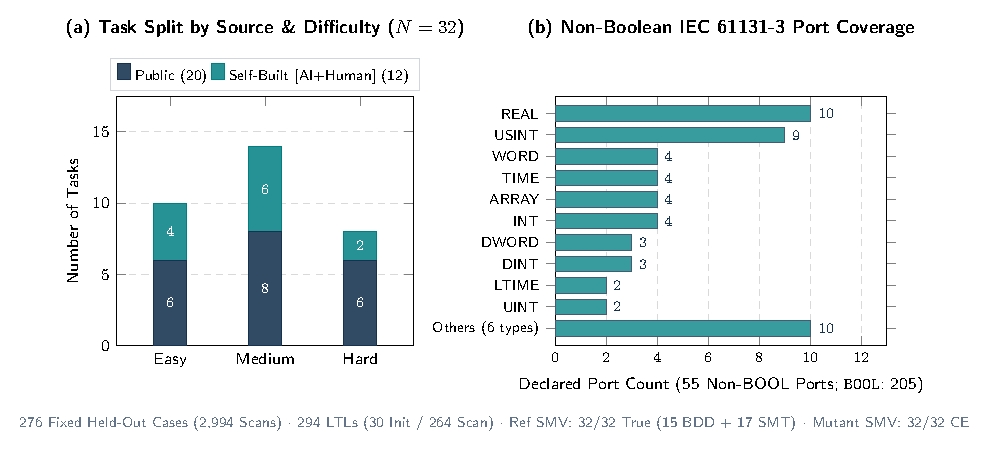
\includegraphics[width=0.98\textwidth]{fig1_dataset_composition.pdf}
  \caption{Dataset composition: (a)~stratified split across source and difficulty tiers ($N=32$); (b)~coverage of 55 non-Boolean IEC~61131-3 ports (excluding 205 \code{BOOL} ports) alongside aggregate trace and SMV dual-control counts.}
  \label{fig:dataset}
\end{figure}

\subsection{Scan-Aligned LTL Corpus and Dual-Control SMV Verification}
The benchmark incorporates \textbf{294 annotated LTL properties} (181 public, 113 self-built) partitioned strictly into two scopes:
\begin{itemize}
  \item \code{INITIAL_INSTANCE} \textbf{(30 formulas, task \code{P_init})}: Constraints checked prior to scan~0 immediately after function-block instantiation (e.g., outputs and retained latches initialized to \code{FALSE}), preventing erroneous application of temporal operator $\mathbf{G}$ across pre-execution states.
  \item \code{SCAN_SEQUENCE} \textbf{(264 formulas)}: Encompasses 50 explicit \code{safety} invariants, transition dynamics, persistent fault latching (expressed via weak-until expansions such as $\mathbf{G}\,Fault \lor (Fault\ \mathbf{U}\ (\neg Jam \land Reset))$ in \code{SELF004} when operator resets may remain idle indefinitely), fairness-guarded conditional liveness, and \code{CompleteBehavior} specifications.
\end{itemize}

Whereas Pre-Scan Moore conventions record outputs on the next cycle ($q[k+1]$), real CODESYS cyclic recorders and this benchmark log \textbf{End-of-Scan Records}:
\begin{equation}
  T[k] = \big(I[k],\; q[k],\; O[k]\big), \qquad q[k+1] = \delta\big(q[k], I[k]\big),\quad O[k] = \lambda\big(q[k], I[k]\big).
\end{equation}
Because scan~$k$'s sampled output $O[k]$ reflects same-scan combinational overrides immediately, safety stop preemption writes cleanly without next-state delay as $\mathbf{G}\big((StopBtn \lor EStop) \rightarrow \neg Motor\big)$, while cross-scan retention references explicit pre-state propositions (e.g., \code{qRun}), keeping discrete runtime traces and SMV models semantically locked.

To verify both specification soundness and fault sensitivity, every task ships an explicit reference SMV model (\pathcode{models/*_reference.smv}) alongside an adversarial mutant SMV injecting realistic logical or timing bugs (\pathcode{models/*_mutant.smv}). Tracked under SHA-256 freshness guarantees by \pathcode{smv_status.py} in \pathcode{configs/smv_verification_status.json}, \textbf{32/32 reference models achieve \code{MODEL_PROPERTIES_TRUE}} (15 \code{NuSMV} BDD + 17 \code{nuXmv} SMT; 285/285 explicit reference properties verified), while \textbf{32/32 negative-control mutant models produce \code{COUNTEREXAMPLE}} (15 BDD + 17 SMT), plus 1 verified \code{complete} BDD model.

\section{The STAR Agent Framework and Supporting Infrastructure}

\subsection{Overview and Leak-Free Architecture}
STAR replaces unstructured free-form agent loops with an artifact-centric multi-stage pipeline operating strictly on a physically scrubbed \code{agent_view()} input (Figure~\ref{fig:arch}). Every benchmark task strips reference implementations, \code{tests}, \code{test_bindings}, \code{specification_contract}, and \code{CompleteBehavior} entries prior to exposing prompts to either STAR or Codex CLI, preserving symmetric zero-leakage conditions until offline evaluation in \pathcode{batch.py}.

\begin{figure}[htbp]
  \centering
  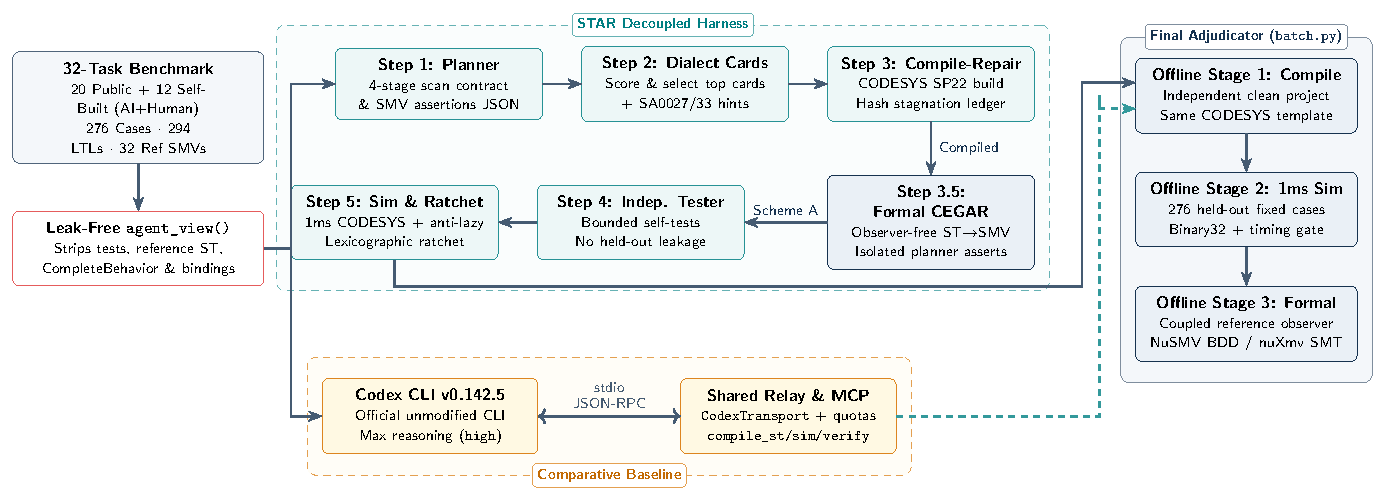
\includegraphics[width=\textwidth]{fig0_star_architecture.pdf}
  \caption{End-to-end architecture comparing the leak-free STAR decoupled pipeline, the symmetric \code{Codex CLI~v0.142.5 + MCP} baseline, and the three-stage offline adjudicator (\pathcode{batch.py}).}
  \label{fig:arch}
\end{figure}

\subsection{Core Design Elements and Engineering Trade-offs}
\begin{enumerate}
  \item \textbf{Task Organization (Step~1 Planner)}: Rather than mixing state-machine partitioning with low-level ST syntax in one generation turn, Step~1 emits a structured JSON scan blueprint specifying state enums, timer/edge instances with reset conditions, priority layers, initial values, and a four-phase deterministic scan skeleton: \code{1) input and edge sampling} $\rightarrow$ \code{2) safety preemption and state transitions} $\rightarrow$ \code{3) unconditional top-level TON/R_TRIG execution} $\rightarrow$ \code{4) post-state output assignment}. Step~3 guarantees timers never freeze inside skipped \code{CASE}/\code{IF} arms, while Steps~2 and~4 prevent intra-scan safety-override conflicts.
  \item \textbf{Context Management Trade-offs (\pathcode{task_view.py}, \pathcode{dialect_cards.py}, \pathcode{harness.py})}:
    \begin{itemize}
      \item \emph{Selective Dialect Cards}: Injecting the complete CODESYS manual wastes context budget and dilutes attention on control logic, whereas omitting dialect nuances invites repeated compiler faults. As a practical trade-off between guidance completeness and prompt focus, STAR curates 8 concise dialect cards (\code{VARIANT}, \code{ARRAY[*]}, \code{LTIME}, unconditional \code{TON}/\code{R_TRIG}, \code{VAR_IN_OUT} structs, 0-based \code{s[i]} vs.\ 1-based \code{STRING} library indexing, and pre-\code{CASE} mode normalization) alongside static-analysis hints, ranking them against interface/text cues and keeping the top-ranked subset (currently top~4).
      \item \emph{Diagnostic Compaction \& Stagnation Ledger}: \code{compact_diagnostics()} extracts localized code snippets and line/column pointers around compiler errors, attaches actionable advice for \code{SA0027} (keyword shadowing) and \code{SA0033} (unused declarations), and pairs with a bounded sliding-window failure log (\code{attempt_ledger}) to curb A$\leftrightarrow$B repair oscillation without unbounded prompt growth.
      \item \emph{First-Divergence Desensitized Feedback}: Both simulation and formal loops feed back only the minimal input prefix up to the first failing scan (\code{first_bad_step}) or shortest counterexample trace.
    \end{itemize}
  \item \textbf{Real Compiler Verification \& Five-Stage \code{ST->SMV} Engine (\pathcode{compiler.py}, \pathcode{st_verifier.py})}:
    \begin{itemize}
      \item \emph{CODESYS Rebuild \& \code{1ms} Replay}: Non-ASCII workspace paths are automatically relocated into ASCII staging directories, builds verify \code{app.generate_code()} static checks, nonces, and template SHA-256 digests, and simulation tests execute isolated \code{FB_Task} test programs via \code{binary32} byte-exact float matching to avoid JSON rounding drift.
      \item \emph{Observer-Free In-Loop Verification (Scheme~A) \& Expression Lowering}: Inside Step~3.5 (and baseline MCP \code{verify_st}), \code{st_verifier.py} parses ST ASTs into pre-init ($t=-1$) and single-scan SSA transition models ($t \ge 0$) with qualified enum resolution and built-in symbolic semantics for 9 standard FBs (\code{TON}, \code{TOF}, \code{TP}, \code{R_TRIG}, \code{F_TRIG}, \code{RS}, \code{SR}, \code{CTU}, \code{CTD}). Built-in \code{_SMVExprParser} and \code{_translate_st_ltl_to_smv} automatically normalize mixed Boolean/relational operators, unfold chained comparisons (e.g., \code{-4 <= x <= 4}), translate typed base literals (\texttt{\small DWORD\#0}, \texttt{\small WORD\#16\#...}), and reject malformed nested temporal expressions prior to invoking BDD/SMT solvers. Crucially, internal generation runs \code{Scheme A} without linking the held-out reference observer (\code{include_expected_observer=False}), while keeping Planner-generated \code{formal_assertions} isolated so malformed planner assertions automatically fall back to benchmark LTLs rather than halting verification. Only frozen final candidates enter Stage~3 coupled reference-observer equivalence checks. Unsupported constructs (e.g., \code{VARIANT}, \code{__VARINFO}) cleanly report \code{UNSUPPORTED_ST} alongside \code{PASS}, \code{COUNTEREXAMPLE}, \code{INCONCLUSIVE}, \code{TIMEOUT}, and \code{TOOL_ERROR}.
    \end{itemize}
  \item \textbf{Repair Loop Engineering Trade-offs \& Termination}:
    When Step~4 constructs self-tests without oracle ground truth, forbidding all test pruning risks misleading repairs from faulty self-tests, while unrestricted pruning risks trivializing tests. STAR enforces a structural constraint---\textbf{\code{lazy_rejection_blocked}}---disallowing case dismissal unless the candidate code hash substantively changes. Candidate acceptance follows a lexicographic 4-tuple \code{(compiled, formal_passed_props, sim_passed_cases, -len(rejected_case_ids))}: if a candidate edit regresses any higher-priority criterion, the ratchet rolls back to the best verified version. The trade-off is favoring reliable local convergence under tight repair budgets over multi-step disruptive refactoring. Finally, infrastructure faults (\code{TOOL_ERROR}, \code{TIMEOUT}, \code{UNVERIFIED}) remain cleanly separated from logical outcomes.
\end{enumerate}

\subsection{Specification Auditing Support and Zero-Dependency WebUI Visualization}
Beyond core synthesis, engineering effort invested substantially in making formal specifications auditable, regressions reproducible offline, and agent traces visually inspectable:

\subsubsection{Multi-Layer Specification Auditing and Offline Regression}
\begin{enumerate}
  \item \textbf{\code{ScanContract} Dual-Mode Offline Regression}: Combines transition-model multi-step contract validation and differential random testing so the core timing and semantic suite runs fast on headless Linux nodes without Windows/CODESYS dependencies.
  \item \textbf{Three-Variant SMV Freshness Tracking (\code{smv_status.py})}: Automatically discovers \code{reference}, \code{complete}, and \code{mutant} SMV files per task, infers \code{bdd} vs.\ \code{smt} solver requirements, probes \code{NuSMV}/\code{nuXmv} binary availability, and hashes model/config state into \pathcode{configs/smv_verification_status.json}, flagging edited artifacts automatically as \code{STALE} (or \code{CHECKER_MISSING}/\code{UNVERIFIED}) so outdated proofs are never reused.
  \item \textbf{Six-Category LTL Symbol Taxonomy (\code{symbol_glossary.py})}: Parses every identifier appearing inside LTL formulas and contracts and assigns it into six semantic classes---\code{input} ($I[k]$), \code{output} ($O[k]$), \code{persistent_inout} (caller-owned \code{VAR_IN_OUT}), \code{obs_history} (prior-scan output $O[k-1]$), \code{ghost_state} (cross-scan reference state, edge memory $I[k-1]$, timer internals), and \code{alias} (combinational/temporal/contract macro aliases)---paired with bilingual definitions to eliminate observer-variable ambiguity during audits.
\end{enumerate}

\subsubsection{Full-Stack Bilingual Industrial WebUI (\code{webui.py} \& \code{run_trace.py})}
Implemented strictly over Python standard-library HTTP services with zero third-party frontend/backend dependencies, the WebUI unifies live backend status diagnostics and four specialized workspaces:
\begin{enumerate}
  \item \textbf{Dataset \& Specs (\code{tab-explorer})}: Supports source/difficulty filtering across all 32 tasks, side-by-side bilingual spec inspection, nested-bracket LTL highlighting with click-to-inspect six-class definitions (\code{spec-popover} powered by \pathcode{symbol_glossary.py}), reference ST/\code{.smv} inspection, and live in-browser \code{NuSMV}/\code{nuXmv} re-verification via \pathcode{/api/check-reference-model}.
  \item \textbf{Agent Workflow (\code{tab-trace} + \pathcode{run_trace.py})}: Safely resolves workspace artifacts inside \pathcode{experiments/} and \pathcode{results/raw/} to reconstruct complete execution timelines---displaying Planner contract JSON, Dialect card selections, per-turn \code{version_*} syntax diffs, compact diagnostics, and CEGAR/simulation repair iterations.
  \item \textbf{Sandbox \& Waveform Lab (\code{tab-sandbox})}: Provides an interactive ST editor with live demo chips connected to \pathcode{/api/evaluate}, \pathcode{/api/verify-candidate}, and \pathcode{/api/export-verify}, plus \code{_build_step_waveforms()} to plot digital square waves and analog step trajectories while highlighting the exact \emph{first-divergence scan} where candidate behavior deviates from expected traces.
  \item \textbf{Benchmark Results (\code{tab-benchmark})}: Aggregates multi-condition experiment summaries via \pathcode{/api/experiments} across overall, public/self-built, and difficulty splits (corresponding directly to the aggregate metrics in Section~5.2).
\end{enumerate}

\clearpage
% Section 5.1 & 5.2: Infrastructure Preflight and Full Four-Condition Empirical Matrix

\section{Empirical Validation, Benchmark Results, and Analysis}

This section reports baseline infrastructure and reference-model preflight validation (Section~5.1), complete quantitative benchmark results across the $2 \times 2$ crossed 128-run matrix (\textbf{E1}--\textbf{E4}, 32 tasks each; Section~5.2), cross-condition diagnostic case studies (Section~5.3), and methodological threats to validity (Section~5.4).

\subsection{Infrastructure and Reference-Model Preflight}
Prior to multi-condition LLM benchmarking, every static validator, toolchain adapter, and reference oracle underwent isolated verification (Table~\ref{tab:preflight}). Because \pathcode{tests/test_webui.py} evolves alongside active UI refinements, core regression checks cover the 27 non-WebUI Python test modules (\code{223/223} passing assertions on current \code{HEAD}).

\begin{table}[htbp]
\centering
\caption{Pre-campaign infrastructure, compiler, static-analysis, and reference-model validation summary.}
\label{tab:preflight}
\footnotesize
\begin{tabularx}{\textwidth}{@{}L{0.20\textwidth}L{0.31\textwidth}Y@{}}
\toprule
\textbf{Verification Check} & \textbf{Command / Evidence} & \textbf{Observed Outcome} \\
\midrule
\textbf{Dataset Integrity} & \code{plc-agent validate-dataset} & 32 tasks (20 public + 12 AI-generated/human-reviewed), 276 cases, 2,994 scans, 294 LTLs; \code{errors=[]}; 1.0 text alignment on 20/20 public tasks. \\
\textbf{Core Unit Test Suite} & \code{unittest} (27 non-WebUI modules) & \textbf{223/223 passed} covering view isolation, relay/budget quotas, decoupled lock timeouts, \code{ST->SMV} lowering, and MCP tooling. \\
\textbf{CODESYS Compile \& SA Probe} & \pathcode{compiler_preflight.json}, \pathcode{static_analysis_preflight.json} & Verified \code{PASS (20.3s)} $\rightarrow$ fault injection \code{C0032/C0046} (\code{COMPILE_FAIL}) $\rightarrow$ recovery \code{PASS (24.7s)}, plus \code{SA0033} gating. \\
\textbf{Reference \& Mutant SMVs} & \pathcode{configs/smv_verification_status.json} & \textbf{32/32} reference SMVs \code{MODEL_PROPERTIES_TRUE} (15 \code{NuSMV} BDD + 17 \code{nuXmv} SMT; \textbf{285/285} properties) and \textbf{32/32} mutants \code{COUNTEREXAMPLE}. \\
\textbf{Reference \code{ST->SMV}} & \pathcode{st_formal_verification.json} & \textbf{14/14 \code{PASS}} on supported fragment (all 12 \code{SELF} + \code{PUB006}/\code{007}); 2 tasks with \code{VARIANT} classified \code{UNSUPPORTED_ST}. \\
\textbf{\code{ScanContract} Regression} & \pathcode{scan_contract_acceptance.json} & 44 contract unit checks + 15 full-task transition verifications passed; \textbf{6/6} injected mutant traces detected as \code{VIOLATED}. \\
\bottomrule
\end{tabularx}
\end{table}

\subsection{Full Four-Condition Matrix Results: E1--E4 Across 128 Runs}
Drawing on the 14~November~2026 unified snapshot (\pathcode{results/summary/fullflow_matrix_snapshot_20261114.json}), resumed \code{Codex CLI} records (\pathcode{results/raw/codex_matrix_resume_20261114/}), and recovered \textbf{E3} workspaces (\pathcode{results/raw/six_task_fullflow_20261114/}), all four conditions (\textbf{E1}--\textbf{E4}) have completed end-to-end synthesis, CODESYS~V3.5 SP22 compilation, real \code{1ms} simulation replay, and Stage~3 coupled \code{ST->SMV} adjudication across all 32 tasks ($128/128$ runs) under maximum reasoning effort (\code{reasoning.effort = "high"}). Table~\ref{tab:benchmark} strictly separates \emph{evaluated} denominators from \emph{planned} denominators (276 fixed cases across 32 tasks) and retains pre-\pathcode{cef1388} \pathcode{TOOL_ERROR} and \pathcode{TIMEOUT} events unaltered.

\begin{table}[htbp]
\centering
\caption{Complete four-condition empirical benchmark summary across 128 runs (32 tasks per condition, as of 14 November 2026).}
\label{tab:benchmark}
\scriptsize
\setlength{\tabcolsep}{4pt}
\begin{tabularx}{\textwidth}{@{}>{\raggedright\arraybackslash}p{0.20\textwidth}YYYY@{}}
\toprule
\textbf{Evaluation Metric} & \textbf{E1: Codex + DeepSeek} & \textbf{E2: Codex + Terra} & \textbf{E3: STAR + DeepSeek} & \textbf{E4: STAR + Terra} \\
\midrule
\textbf{Completed Tasks} & \textbf{32/32} (uniform audit) & \textbf{32/32} (uniform audit) & \textbf{32/32} (uniform audit) & \textbf{32/32} (uniform audit) \\
\textbf{First-Pass Compile} & 23/32 (71.9\%); +5 repaired (18 repairs, 50 calls) & 26/32 (81.2\%); +3 repaired (4 repairs, 36 calls) & \textbf{27/32 (84.4\%)}; +5 repaired (5 repairs, 40 calls) & \textbf{27/32 (84.4\%)}; +1 repaired (3 repairs, 39 calls) \\
\textbf{Final Compilation} (All / \texttt{SELF} / \texttt{PUB}) & \textbf{28/32 (87.5\%)} (\texttt{S} 11/12, \texttt{P} 17/20; 4 \texttt{SA0027}) & \textbf{29/32 (90.6\%)} (\texttt{S} 12/12, \texttt{P} 17/20; 1 \texttt{FAIL}, 2 \texttt{TE}) & \textbf{32/32 (100.0\%)} (\texttt{S} 12/12, \texttt{P} 20/20) & \textbf{28/32 (87.5\%)} (\texttt{S} 12/12, \texttt{P} 16/20; 1 \texttt{FAIL}, 3 \texttt{TE}) \\
\textbf{Fixed Cases (Eval.\ Denom.)} & \textbf{196/208 (94.2\%)} (\texttt{S} 92/92, \texttt{P} 104/116) & \textbf{220/222 (99.1\%)} (\texttt{S} 99/99, \texttt{P} 121/123) & \textbf{226/238 (95.0\%)} (\texttt{S} 99/99, \texttt{P} 127/139) & \textbf{217/221 (98.2\%)} (\texttt{S} 99/99, \texttt{P} 118/122) \\
\textbf{Fixed Cases (Planned 276)} & \textbf{196/276 (71.0\%)} & \textbf{220/276 (79.7\%)} & \textbf{226/276 (81.9\%)} & \textbf{217/276 (78.6\%)} \\
\textbf{Task Functional Pass} (All / Eval.) & \textbf{23/32 (71.9\%)}; 23/27 (85.2\%) (\texttt{S} 11/12, \texttt{P} 12/20) & \textbf{27/32 (84.4\%)}; \textbf{27/29 (93.1\%)} (\texttt{S} 12/12, \texttt{P} 15/20) & \textbf{27/32 (84.4\%)}; 27/31 (87.1\%) (\texttt{S} 12/12, \texttt{P} 15/20) & \textbf{25/32 (78.1\%)}; 25/28 (89.3\%) (\texttt{S} 12/12, \texttt{P} 13/20) \\
\textbf{Tier Task Pass} (\texttt{E10}/\texttt{M14}/\texttt{H8}) & 7/10 (70.0\%) $\cdot$ 11/14 (78.6\%) $\cdot$ 5/8 (62.5\%) & 10/10 (100.0\%) $\cdot$ 13/14 (92.9\%) $\cdot$ 4/8 (50.0\%) & 9/10 (90.0\%) $\cdot$ 13/14 (92.9\%) $\cdot$ 5/8 (62.5\%) & 8/10 (80.0\%) $\cdot$ 13/14 (92.9\%) $\cdot$ 4/8 (50.0\%) \\
\textbf{Stage~3 Formal} (\texttt{ST->SMV})$^{a}$ & \texttt{PASS} 16 (\texttt{S}11+\texttt{P}5); \texttt{CE} 3; \texttt{TO} 1; \texttt{UNSUP} 8; \texttt{NR} 4 & \textbf{\texttt{PASS} 18} (\texttt{S}12+\texttt{P}6); \texttt{CE} 1; \texttt{TO} 1; \texttt{UNSUP} 9; \texttt{NR} 3 & \texttt{PASS} 17 (\texttt{S}12+\texttt{P}5); \texttt{CE} 3; \texttt{UNSUP} 12; \texttt{TO}/\texttt{NR} 0 & \textbf{\texttt{PASS} 18} (\texttt{S}12+\texttt{P}6); \texttt{CE} 1; \texttt{TO} 1; \texttt{UNSUP} 8; \texttt{NR} 4 \\
\textbf{Adjudicator Verdicts} (\pathcode{batch.py}) & \texttt{PARTIAL} 20, \texttt{FAIL} 10, \texttt{TO} 1, \texttt{TE} 1 & \texttt{PARTIAL} 26, \texttt{FAIL} 3, \texttt{TO} 1, \texttt{TE} 2 & \texttt{PARTIAL} 26, \texttt{FAIL} 5, \texttt{TE} 1 & \texttt{PARTIAL} 24, \texttt{FAIL} 4, \texttt{TO} 1, \texttt{TE} 3 \\
\textbf{Gen.\ Calls \& In-Loop Tools} & 184 reqs (50 compile / 9 sim / 37 verify) & 93 reqs$^{b}$ (36 compile / 1 sim / 1 verify) & 104 reqs (40 compile / 34 sim / 32 verify) & 99 reqs (39 compile / 32 sim / 28 verify) \\
\textbf{Tokens (32/32 Tasks)} & 4,742,114 in (85.6\% cached) / 515,786 out (331,389 reas.) & 1,260,812 in (58.9\% cached) / \textbf{72,823 out} (20,979 reas.) & 432,953 in (17.3\% cached) / 778,596 out (651,225 reas.) & \textbf{365,578 in} (11.2\% cached) / 215,832 out (125,818 reas.) \\
\textbf{API Cost \& Gen.\ Latency}$^{b}$ & \textbf{\textyen 2.15}; mean 143.5\,s (med.\ 107.0\,s) & \textbf{\textyen 5.21}; mean \textbf{91.0\,s} (med.\ 66.1\,s) & \textbf{\textyen 2.74}; mean 218.2\,s (med.\ 171.5\,s) & \textbf{\textyen 7.38}; mean 129.2\,s (med.\ 98.1\,s) \\
\bottomrule
\end{tabularx}
\par\vspace{3pt}
\raggedright\scriptsize
$^{a}$ Abbreviations: \texttt{S}/\texttt{P} = \texttt{SELF}/\texttt{PUB}; \texttt{CE} = \texttt{COUNTEREXAMPLE}; \texttt{TO} = \texttt{TIMEOUT}; \texttt{TE} = \texttt{TOOL\_ERROR}; \texttt{UNSUP} = \texttt{UNSUPPORTED\_ST}; \texttt{NR} = \texttt{NOT\_RUN}. Timed test cases exceeding practical wall-clock bounds or zero-tolerance host timing limits, plus uncompiled or harness-incompatible tasks, are excluded from evaluated-denominator percentages rather than marked as passes.\\
$^{b}$ Generation telemetry covers all 32 tasks per group (\textbf{E3} includes the 6 recovered tasks under \pathcode{results/raw/six_task_fullflow_20261114/}, totaling 104 requests and \textyen 2.74). Provider cost is absent on 1 of 184 requests in \textbf{E1}, and token/cost usage fields are absent on 10 of 93 requests in \textbf{E2}.
\end{table}
\IfFileExists{results_interpretation.tex}{% Section 5.2 (Visual Breakdown & Observations)

\subsubsection{Visualizing Empirical Trade-Offs and Key Observations}
\label{sec:results_interp}

Figures~\ref{fig:overview}--\ref{fig:tokens} dissect the empirical profile across all four experimental conditions (\textbf{E1}--\textbf{E4}, 128 runs total) by aggregate split metrics, difficulty scaling, Stage~3 formal outcomes, and generation efficiency.

\begin{figure}[htbp]
  \centering
  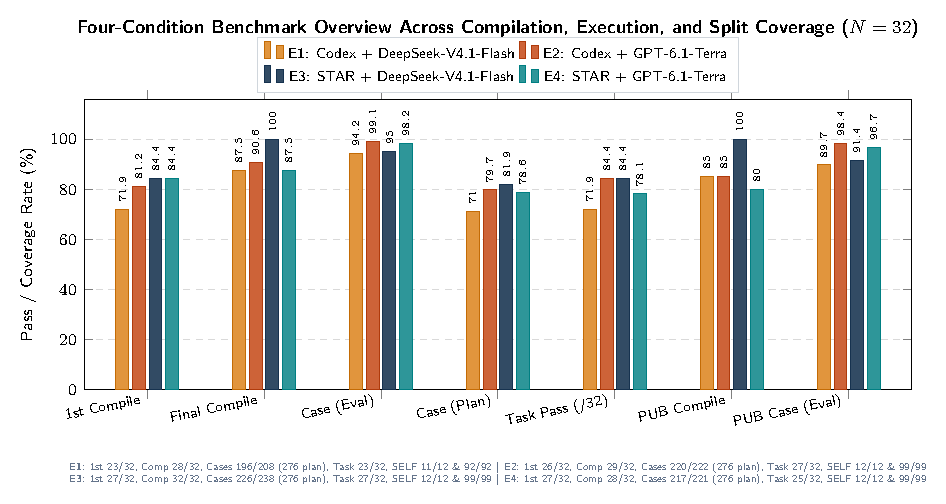
\includegraphics[width=0.98\textwidth]{fig2_four_group_overview.pdf}
  \caption{Cross-condition comparison across \textbf{E1} (Codex + DeepSeek), \textbf{E2} (Codex + Terra), \textbf{E3} (STAR + DeepSeek), and \textbf{E4} (STAR + Terra) covering first-pass and final compilation, evaluated vs.\ planned fixed cases, task-level pass rate, and \code{public} ($n=20$) vs.\ \code{self_built} ($n=12$) splits.}
  \label{fig:overview}
\end{figure}

\begin{figure}[htbp]
  \centering
  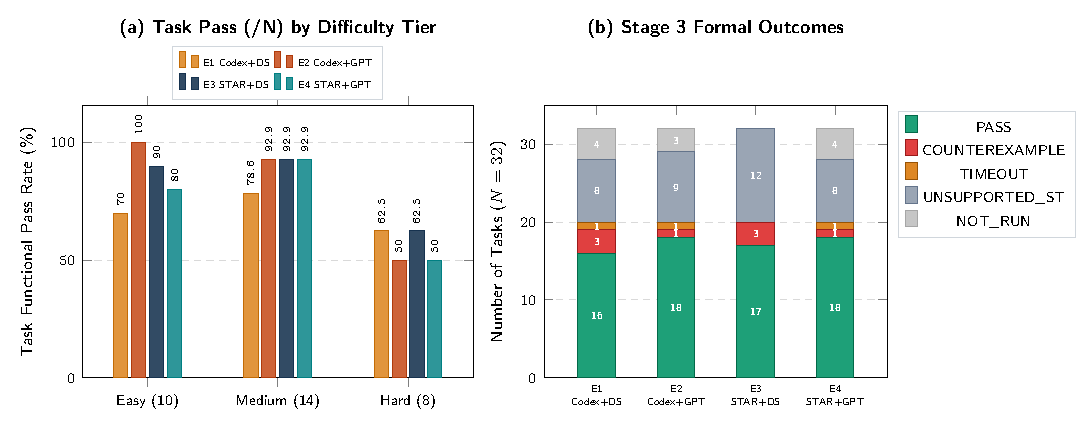
\includegraphics[width=0.98\textwidth]{fig3_difficulty_formal_breakdown.pdf}
  \caption{Stratified performance and formal diagnosis across \textbf{E1}--\textbf{E4}: (a)~task-level functional pass rate across Easy ($n=10$), Medium ($n=14$), and Hard ($n=8$) tiers; (b)~Stage~3 formal \code{ST->SMV} outcome counts ($N=32$ tasks per condition).}
  \label{fig:breakdown}
\end{figure}

\begin{figure}[htbp]
  \centering
  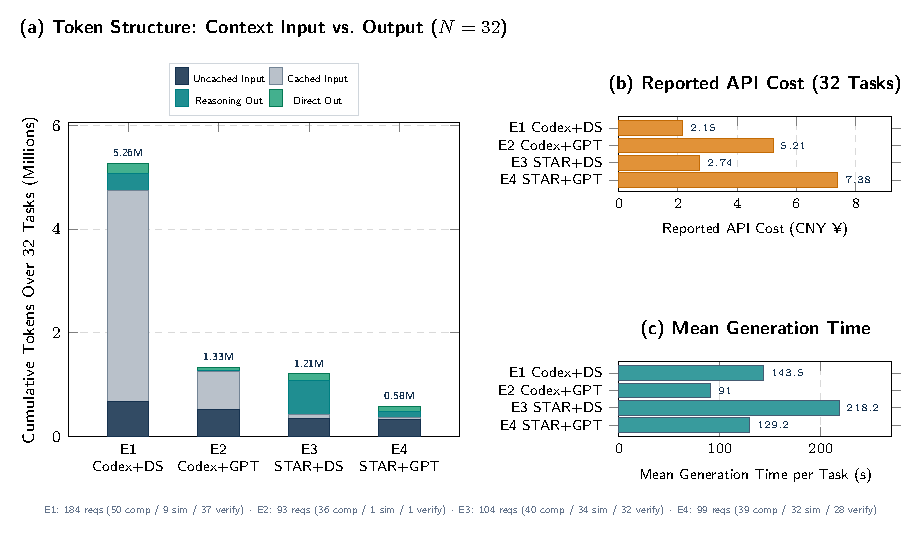
\includegraphics[width=0.96\textwidth]{fig4_token_cost_efficiency.pdf}
  \caption{Generation resource efficiency across \textbf{E1}--\textbf{E4} ($N=32$ tasks per condition): (a)~cumulative 32-task input tokens (cached vs.\ uncached) and output tokens (reasoning vs.\ direct emission); (b)~total reported provider API cost (RMB); (c)~mean generation elapsed time per task (s).}
  \label{fig:tokens}
\end{figure}

Four consistent empirical findings emerge from Table~\ref{tab:benchmark} and Figures~\ref{fig:overview}--\ref{fig:tokens}:
\begin{enumerate}
  \item \textbf{Framework Benefit Depends Sharply on Foundation Model Capability (\textbf{E3} vs.\ \textbf{E1})}: On \code{deepseek-v4.1-flash-1017}, unguided \code{Codex CLI} (\textbf{E1}) issues 184 LLM requests and 50 compiles, accumulating 4,742,114 input tokens (4,057,344 cached, 684,770 uncached) across multi-turn agent transcripts, yet stalls at \textbf{28/32 (87.5\%)} compilation, 196/208 (94.2\% evaluated; 71.0\% planned) fixed cases, and 23/32 (71.9\%) task passes with 10 functional failures. Under \textbf{STAR} (\textbf{E3}), view isolation, targeted dialect cards, and compact diagnostics raise compilation to \textbf{32/32 (100.0\%)}, lift evaluated cases to 226/238 (and peak planned coverage at \textbf{81.9\%}), boost task passes to 27/32 (halving \code{FAIL} outcomes to 5), and compress total input volume roughly \textbf{11$\times$} to 432,953 tokens (104 requests).
  \item \textbf{Structured Multi-Role Pipeline vs.\ Unconstrained Tool-Use on Stronger Models (\textbf{E2} vs.\ \textbf{E4})}: On \code{gpt-6.1-terra}, unconstrained \code{Codex CLI} (\textbf{E2}) rarely requires exploratory recovery (triggering only 1 in-loop simulation and 1 formal call across all 32 tasks), achieving \textbf{29/32 (90.6\%)} compilation, the matrix-high \textbf{99.1\% (220/222)} evaluated case pass rate, and \textbf{27/32} task passes (27/29 = 93.1\% evaluated) with minimal 72,823 total output tokens, \textyen 5.21 cost, and 91.0\,s mean generation latency. Under \textbf{STAR} (\textbf{E4}), the model achieves the same \textbf{18} Stage~3 formal \code{PASS} verdicts and lowest input footprint (365,578 tokens), but mandatory multi-stage JSON Planning, Coding, and Testing inflate total output tokens nearly $3\times$ (215,832), raising cost to \textyen 7.38 and mean latency to 129.2\,s while passing two fewer tasks overall (one extra \code{FAIL} on \code{PUB004} and one extra lock timeout on \code{PUB006}). Fixed heavy orchestration therefore adds output overhead on models already strong enough to compile cleanly, motivating adaptive difficulty-gated routing.
  \item \textbf{High Reliability on Self-Built Control Suite (\code{SELF001}--\code{SELF012})}: Across \textbf{E2}, \textbf{E3}, and \textbf{E4}, all three conditions achieve \textbf{12/12 compilation, 99/99 fixed-case pass, and 12/12 Stage~3 formal verification pass}. Across all 48 self-built runs in the $2 \times 2$ matrix, only one run failed---\textbf{E1}/\code{SELF009}---solely due to omitting CODESYS static-analysis dialect guardrails (\code{SA0027}).
  \item \textbf{Lock Contention Dominates GPT Compilation Gaps and \code{PARTIAL} Bounds Reflect Execution Scope}: Beyond \code{PUB018} (\code{VARIANT} reflection), all uncompiled tasks in \textbf{E2} (\code{PUB014}, \code{PUB017}) and \textbf{E4} (\code{PUB006}, \code{PUB014}, \code{PUB017}) terminated as infrastructure \code{TOOL_ERROR}s from compiler mutex contention (\code{Compiler lock wait deadline exceeded}), directly prompting commit \pathcode{cef1388} to decouple lock wait deadlines from compile timeouts. Separately, \code{PARTIAL} verdicts in \pathcode{batch.py} stem from physical hour-scale timer exclusions and explicit \code{UNSUPPORTED_ST} lowering exits rather than silent falsification.
\end{enumerate}}{}
\FloatBarrier
% Section 5.3: Deep-Dive Case Studies Across E1-E4

\subsection{Deep-Dive Case Studies}

\subsubsection{Case Study 1: Hidden Single-Scan Delay Masked by 100\% Simulation Pass (\code{PUB011})}
\code{PUB011} specifies a three-station transfer trolley toggling between manual and automatic operation. Cross-condition inspection contrasts both runtime-vs.-formal coverage and per-run synthesis variance:
\begin{itemize}
  \item \textbf{E3 Passes 8/8 Fixed Tests Yet Fails 8/14 NuSMV Properties}: DeepSeek under STAR (\pathcode{results/raw/four_group_20261114/star_deepseek_v3/PUB011/generation/compile_00/FB_Task.st}) achieves \textbf{8/8 (100\%)} pass on real CODESYS~1\,ms simulation tests. During Stage~3 verification, however, \code{NuSMV} proves only 6/14 LTLs and builds deterministic counterexamples against 8 transition obligations (incl.\ \code{SMV_4}, \code{SMV_8}, \code{SMV_9}) due to an intermediate \code{E_Phase.MANUAL} state inserted before the dispatcher:
\begin{lstlisting}[caption={Relevant E3 (\code{PUB011}) mode-switch logic introducing a one-scan startup delay.},float=htbp]
IF NOT Mode THEN
    phase := E_Phase.MANUAL;
ELSIF phase = E_Phase.MANUAL THEN
    phase := E_Phase.WAIT_A;
ELSE
    CASE phase OF ...
\end{lstlisting}
  On the exact rising-edge scan transitioning from \code{Mode = FALSE} to \code{TRUE} with \code{SensorA} and \code{ButtonA} asserted, one scan is spent resetting \code{phase} from \code{MANUAL} to \code{WAIT_A}, delaying \code{MotorForward} by one scan cycle---a corner case never triggered by the 8 finite test sequences.
  \item \textbf{E1, E2, and E4 Preserve Same-Scan Entry Semantics}: By contrast, \textbf{E4} (\pathcode{results/raw/four_group_20261114/star_terra/PUB011/generation/compile_00/FB_Task.st}, maintaining \code{E_TaskPhase.WAIT_A} during \code{NOT Mode}) as well as both \code{Codex CLI} baselines (\textbf{E1} and \textbf{E2}) stay directly in their \code{WAIT_A} phase while in manual mode, allowing immediate same-scan transition and simultaneously passing \textbf{8/8 simulation cases and 14/14 formal LTLs}.
\end{itemize}

\subsubsection{Case Study 2: Universal Transient Latching and Priority Arbitrations (\code{PUB019})}
On the 18-input, 6-output multi-mode robotic arm controller \code{PUB019} (Hard), \textbf{all four conditions (\textbf{E1}--\textbf{E4}) converge on the exact same residual flaw}: every group scores \textbf{16/17} on fixed cases, failing exclusively at scan~1 of \code{PUB019.T6} (\code{MoveUp} expected \code{TRUE}, measured \code{FALSE}), and every group terminates with Stage~3 \code{COUNTEREXAMPLE} (\textbf{E1}: 4/8, \textbf{E2}: 3/8, \textbf{E3}: 5/10, \textbf{E4}: 6/10 properties satisfied). Two common failure mechanisms explain this convergence:
\begin{enumerate}
  \item \textbf{Over-Suppression on Entry From Idle}: At scan~0 of \code{PUB019.T6}, no mode is active; scan~1 raises \code{ManualMode} alongside \code{UpButton}. Across all four conditions, models detect \code{modeChanged} against quiescent idle state and blank actuator outputs for one scan, rather than gating only active-to-active mode switches.
  \item \textbf{Conservative Mutual Lockout vs.\ Manual Preemption}: When \code{ManualMode} and an auto-mode selector activate concurrently, all four candidates apply \code{modeCount > 1} to freeze all axes safely, whereas the specification's observer defines explicit manual override precedence, triggering immediate scan-0 formal counterexamples.
\end{enumerate}

\subsubsection{Case Study 3: Formal Catch on Bare Codex (\code{PUB020}), Model Divergence (\code{PUB016}), and Indexing Nuance (\code{PUB014})}
\begin{itemize}
  \item \textbf{\code{PUB020} (Multi-Station Production Line)}: Both \code{gpt-6.1-terra} conditions (\textbf{E2} and \textbf{E4}) pass \textbf{11/11 fixed cases and Stage~3 \code{PASS}}. Conversely, both DeepSeek runs draw Stage~3 counterexamples: critically, \textbf{E1} passes \textbf{all 11/11 finite simulation cases} yet satisfies only 3/11 \code{NuSMV} properties (exposing mutual-exclusion violations in \code{REJECT} reachable states, complementing \textbf{E3}/\code{PUB011}), while \textbf{E3} drops late progression in \code{PUB020.T9} (\code{10/11} cases, \code{3/10} formal).
  \item \textbf{\code{PUB016} (Analog Ramp/Step Control)}: Inverting overall model rank order, both DeepSeek groups (\textbf{E1} and \textbf{E3}) pass \textbf{8/8} tests, whereas both GPT groups (\textbf{E2} and \textbf{E4}) fail identically on \code{PUB016.T4} (\textbf{7/8}).
  \item \textbf{\code{PUB014} (Dotted-Decimal IPv4 Parser)}: Both DeepSeek runs (\textbf{E1} and \textbf{E3}) compile on the first attempt yet score \textbf{0/8} at runtime because indexing \code{ipText[i]} defaults to 1-based \code{1..LEN(ipText)} instead of CODESYS's \textbf{0-based} \code{STRING} byte offset \code{s[i]}, reading past the terminator and clearing output. (Both GPT conditions hit compiler-lock timeouts before simulation.) Targeted updates to \pathcode{dialect_cards.py} subsequently codify this 0-based vs.\ 1-based distinction explicitly.
\end{itemize}

\subsubsection{Case Study 4: Vendor Static-Analysis Guardrails (\code{SA0027}/\code{SA0033}) and Generic Reflection (\code{PUB018})}
\begin{itemize}
  \item \textbf{Same-Root \code{SA0027} Elimination Across \textbf{E1} vs.\ \textbf{E3}}: All four compilation failures in \textbf{E1} (\code{Codex + DeepSeek}: \code{PUB003}, \code{PUB009}, \code{PUB017}, \code{SELF009}) failed on the exact same CODESYS static-analysis collision---\code{SA0027} (\code{Variable name 'error' in 'FB_Task'} \code{already used for an object in Library} \code{'caa device diagnosis, 3.5.22.0'}), compounded by \code{SA0033} on \code{PUB017}---despite multiple multi-turn repair iterations. By contrast, \textbf{E3} (\textbf{STAR} + DeepSeek) compiled \textbf{4/4 with zero \code{SA0027} failures} (three on first attempt, \code{PUB017} after one repair) via dialect cards and \code{compact_diagnostics()}, while \textbf{E2} (\code{Codex + Terra}) resolved the first three after 1--2 iterative fixes.
  \item \textbf{\code{PUB018} (Generic Circular Byte Queue)}: Binding caller-owned \code{DINT} variables and fixed arrays via \code{VAR_IN_OUT VARIANT} / \code{VAR_INFO} marks an infrastructure and abstraction frontier: GPT conditions (\textbf{E2}, \textbf{E4}) hit \code{COMPILE_FAIL} (\code{Unknown type: 'VARIANT'}), whereas DeepSeek conditions (\textbf{E1}, \textbf{E3}) compile cleanly yet incur external harness \code{TOOL_ERROR} during simulation type binding.
\end{itemize}
\section{Limitations and reflection}

The most important distinction is between an executed agent run, a compiled candidate and a behaviorally checked controller. A relay outage prevents compilation without demonstrating a syntax error. A successful build can still change an interface or fail a scan trace. Even complete fixed-test success does not prove every input sequence or unbounded LTL liveness.

The automatic runtime adapter has a deliberate coverage boundary: scalar, untimed interfaces. It does not validate physical timing, caller-owned composite storage or the generic FIFO contract. Those tasks retain manual procedures and expected results. The current project does not claim a completed manual campaign, PLCVerif integration, certification, physical PLC deployment or additional-platform support. The reference exploration concerns selected Python-model predicates only.

One observation per task/condition is inadequate for separating model randomness, relay stability and framework effects. The tasks mix source groups and difficulty levels, and only three compile failures were recovered in the observed campaign. Differences in internal prompts, context and the baseline's final-answer request remain framework effects. Both agents see test expectations. Claims about hidden-test generalization or universal superiority would go beyond this design.

The exact identifiers are provider routes. Upstream identities, context sizes and prices could not be independently established. Reported token totals are partial observations, not complete billing estimates. Raw interruption events and usage gaps are retained. A future uniform retry policy or repeated campaign would need to be declared before selecting replacement results.

The requested IDE screenshot could not be acquired through the desktop app-opening permission workflow during this run. The report therefore labels actual diagnostic text as text evidence, preserves the real CODESYS projects and logs, and does not manufacture a GUI screenshot. This presentation limitation does not replace or weaken the compiler checks, but remains an explicitly incomplete requested artifact. A manual screenshot can be added by opening a preserved project in the installed IDE and rebuilding it.

\section{Reproduction and deliverable checks}

The source package retains task builders, specifications, manual tests, configuration, agent adapters, CODESYS scripts and the manifest-selected raw records. Source and result hashes allow independent checks; historical absolute paths are resolved against the extracted project root where supported. Reproduction requires an installed CODESYS profile/template and private API credentials. Commands are documented for PowerShell, with \pathcode{scripts/run.ps1} selecting Project1.

The offline suite passes 38 tests covering dataset validation, status accounting, bounded repair flow, actual baseline integration with controlled transport doubles, evidence hashing/path containment, scalar adapter construction, scan isolation and Python reference consistency. Test doubles live in temporary unit-test directories and never enter benchmark totals. The actual valid--invalid--repaired compiler preflight and actual simulator integration checks provide separate external-system evidence.

The final analysis is reproducible with \pathcode{scripts/analyze_results.py}; the release audit verifies compiler evidence, task/source hashes, denominators, trace evidence, artifact QA and secret exclusion. The final ZIP contains neither the Conda environment nor API credentials. PDF pages and slide previews are visually reviewed, and PPTX object structure is checked for editable text and shapes. A generated explanation video is verified from the actual media duration and decoded fully; its narration is identified as computer generated.

\section{Conclusion}

We implemented a working ST coding harness connected to the actual CODESYS compiler and a real IDE-simulation test adapter, then compared it with an established tool-using agent using two verified relay routes. The preserved repair examples demonstrate that compiler feedback can lead to a successful build, while the FIFO example shows why build success alone is insufficient. The resulting benchmark is useful because failures, unsupported cases and evidence boundaries remain visible. Extending controlled timing and composite-interface testing, then repeating the campaign, would improve its coverage and statistical reliability.

\begin{thebibliography}{9}
\bibitem{codesys-cli} CODESYS, \emph{Starting Scripts from the Command Line}. \url{https://content.helpme-codesys.com/en/CODESYS%20Scripting/_cds_starting_script_via_command_line.html}.
\bibitem{codesys-application} CODESYS, \emph{ScriptApplication API}. \url{https://content.helpme-codesys.com/en/ScriptingEngine/ScriptApplication.html}.
\bibitem{codesys-system} CODESYS, \emph{ScriptSystem API}. \url{https://content.helpme-codesys.com/en/ScriptingEngine/ScriptSystem.html}.
\bibitem{smolagents} Hugging Face, \emph{smolagents Agent Reference}. \url{https://huggingface.co/docs/smolagents/en/reference/agents}.
\end{thebibliography}


\end{document}
